\documentclass[ENG]{TFUOC}

\usepackage{graphicx}
\usepackage{float}
\usepackage{tikz}
\usepackage{booktabs}
\usepackage{array}
\usepackage{multirow}
\usepackage{amsmath}
\usetikzlibrary{arrows.meta,shapes.geometric,positioning,fit,backgrounds,calc}

%Introduce Work Data
\title{Analítica avanzada sobre datos de plataformas VOD y generadores de contenidos en redes sociales}
\titcrt{Analítica de plataformas VOD} %Short title to appear in header
\author{Pablo Jiménez Cruz}
\date{December 2026}


\nomPDC{Francesc Julbe López}
\nomPRA{Appoint Responsible Teaching Staff}
\titulac{Master in Data Science}
\area{Data Science}
\idioma{English}
\credits{12}
\parcla{artificial intelligence, video podcasts, YouTube analytics, automatic speech recognition, speaker diarization, video chaptering, highlight detection, local machine learning}

\licenc{ccBy}

%%%%%%%%%%
% Summary in language

\abstractenglish{
Publishing a long-form video podcast on YouTube requires a series of repetitive post-production tasks (subtitles, chapters, short-form clips, descriptions) and a number of editorial decisions, such as which moments deserve a clip or whether a title and thumbnail will attract clicks, that are usually taken without quantitative support. Existing tools address these tasks in isolation, rely on paid cloud services, and do not learn from the creator's own performance data.

This Final Master's Project presents the design and development of \textit{YouTube Suite}, a self-hosted platform that turns a raw podcast recording into the artefacts YouTube expects and progressively replaces editorial guesswork with models trained on real data. The platform integrates eight tools: transcription and subtitle generation (faster-whisper), speaker diarization (pyannote.audio), chapter generation with locally trained models, show-notes drafting with a local large language model, a transcript-based relevance model, an automatic Shorts generator, a title/thumbnail click-through-rate predictor, and a hook-strength scorer. A market-analysis pipeline collects public data from curated podcast channels and private analytics (retention and real click-through rate) from the operator's own channel, which feed a model retraining loop.

The system is built on FastAPI, PostgreSQL, an asynchronous job queue (arq over Redis) and an Angular front end, and runs entirely on consumer hardware (a 3\,GB GPU) without paid APIs. Development followed a sixteen-milestone plan, each milestone split into planning, development and testing sub-phases, with every architectural choice recorded in dated decision records and every hardware assumption verified by measured experiments. The report describes the state of the art, the architecture and methods of each component, the training of the custom models, and an economic evaluation of the self-hosted approach.
}

\begin{document}

\estructura

\tableofcontents

\listoffigures

\listoftables


%==========================================================
\chapter{Introduction}
%==========================================================

\section{Context and justification of the project}

Over the last decade, video-on-demand (VOD) platforms have become the main distribution channel for audiovisual content, and YouTube in particular has become one of the leading platforms for podcasts, which are increasingly recorded and published as video. Content discovery on these platforms is governed by recommendation systems that optimise engagement signals such as watch time and click-through rate (CTR) \cite{recommender_systems_streaming, vod_bigdata}. As a consequence, the success of an episode depends not only on its content but also on how it is packaged: subtitles, chapters, title, thumbnail, description and short-form clips that act as entry points to the full episode.

For a small production team, preparing this material is costly and repetitive. A one-hour episode requires a synchronised transcript, speaker attribution, chapter markers, several vertical clips, and a description with tags. Moreover, the decisions with the largest impact on reach, namely which moments are worth clipping and which title and thumbnail will be clicked, are usually taken by intuition. The platform provides the data needed to learn from past performance (public statistics through the YouTube Data API, retention curves through the Analytics API and, since January 2026, real thumbnail impressions and CTR through the Reporting API \cite{yt_data_api}), but this data is rarely connected back to the production process.

The commercial tools available in this space (automatic clipping, captioning or title-testing services) solve isolated steps, are offered as paid cloud services that require uploading unpublished material to third parties, and do not train on the creator's own results. Open-source projects cover the mechanical parts (transcription, cropping, caption burn-in) but, as the prior-art review in Chapter~\ref{ch:soa} shows, none of them trains a dedicated model to score the relevance of transcript segments.

This project addresses that gap with \textit{YouTube Suite}, an integrated platform for video-podcast producers built around three principles:
\begin{enumerate}
\item \textbf{Integration}: a single workflow in which every tool reads from and writes to the same data model, so that artefacts produced by one tool (e.g.\ the transcript) are reused by all the others.
\item \textbf{Local execution}: all models, including the language models, run on the operator's own hardware, which keeps unpublished material private and avoids per-use costs.
\item \textbf{Data feedback}: a market-analysis pipeline accumulates real performance data that is used to train and progressively improve the platform's custom models.
\end{enumerate}

%--------------------------------------------------
\section{Objectives of the project}

\subsection*{General objective}

To design, implement and validate a self-hosted platform that automates the post-production of YouTube video podcasts and supports editorial decisions with machine learning models trained on real performance data, running entirely on consumer hardware.

\subsection*{Specific objectives}

\begin{enumerate}
\item Build a modular back end (REST API, relational database and asynchronous job pipeline) in which each AI tool is an independent, traceable job.
\item Implement accurate transcription with word-level timestamps and downloadable subtitles (SRT/WebVTT), and speaker diarization integrated into the transcript and subtitles.
\item Develop a bilingual (English/Spanish) chapter generator based on models trained locally, and evaluate it against an unsupervised baseline with standard segmentation metrics.
\item Generate show notes (title suggestions, description, tags and summary) with a local language model and validated structured output.
\item Design a transcript-based relevance model and use it to generate vertical short-form clips automatically (boundary selection, subject-tracking crop and optional burned-in captions).
\item Build a market-analysis pipeline that collects public data from a curated list of podcast channels and private analytics (engagement, retention and real CTR) from the operator's own channel, within the API quota limits.
\item Implement a title/thumbnail CTR predictor and a hook-strength scorer, bootstrapped with heuristics and designed to be trained with ranking objectives as labelled data accumulates.
\item Provide a model versioning and retraining pipeline in which a trained model replaces its heuristic predecessor only after it demonstrably outperforms it.
\item Expose all functionality through a web interface, and verify every component with automated tests and a regression suite.
\item Evaluate the economic cost and viability of the self-hosted approach.
\end{enumerate}

%--------------------------------------------------
\section{Impact on sustainability, ethical-social aspects and diversity}
\label{s:etic}

This project integrates the Competence of Ethical and Global Commitment (CCEG) following the transversal guidelines for Final Projects. The reflection is structured around the three required dimensions.

\subsection*{Sustainability}

The main environmental impact comes from the energy consumed by model inference and training. The design reduces it in several ways, aligned with SDG~9 (Industry, Innovation and Infrastructure) and SDG~12 (Responsible Consumption and Production):
\begin{itemize}
\item \textbf{Reuse of artefacts.} Audio is extracted once and stored; the transcript is computed once and reused by diarization, chapters, show notes, relevance scoring and clip captions.
\item \textbf{Small, frozen models.} Custom models are lightweight heads trained on top of frozen pretrained encoders, and trainings last minutes to hours on a single consumer GPU instead of large-scale clusters.
\item \textbf{Reuse of existing hardware.} The platform runs on a six-year-old desktop computer with a 3\,GB GPU; model sizes and quantisation were chosen to fit this hardware rather than to require new equipment.
\item \textbf{Efficient data collection.} Public data is collected with batched API calls and free RSS feeds, avoiding continuous polling.
\end{itemize}

\subsection*{Ethical behaviour and social responsibility}

Data collection uses only official YouTube APIs, public data from channels, and private analytics from the operator's own channel under OAuth consent, with credentials encrypted at rest. The training data for the chapter models (VidChapters-7M \cite{yang2023vidchapters}) is derived from public YouTube videos whose rights remain with their authors; it is used only to train models for internal use and is never redistributed. Processing everything locally means that unpublished episodes and guests' voices are never sent to third-party services.

The main ethical risk is the optimisation of content purely for engagement metrics, and the production of decontextualised clips. The platform mitigates this in two ways: it never publishes anything by itself (every artefact is reviewed and published manually by the operator), and its scoring models expose interpretable outputs (e.g.\ the feature contributions of the hook scorer) instead of opaque rankings. This supports SDG~8 (Decent Work and Economic Growth) by reducing repetitive work for small creators while keeping editorial control in human hands.

\subsection*{Diversity, gender and human rights}

Speech recognition, diarization and language models may perform unevenly across accents, languages and voices because of biases in their training data. Two measures address this: the chapter models are explicitly evaluated on a held-out Spanish test set in addition to English, and speaker labels are anonymous (\texttt{SPEAKER\_00}, \texttt{SPEAKER\_01}, \dots), so no identity or gender is inferred from a voice. On the positive side, automatic subtitles improve accessibility for deaf and hard-of-hearing viewers, and bilingual support for Spanish, a language underrepresented in public chaptering datasets, contributes to SDG~10 (Reduced Inequalities). A known limitation is that the text encoders of the v1 relevance, CTR and hook models are English-only; multilingual encoders are identified as future work.

%--------------------------------------------------
\section{Approach and method followed}

The project followed a plan-driven incremental methodology in two stages.

\textbf{Design stage.} Four phases preceded any implementation: (i)~\textit{scope definition}, in which each candidate tool was discussed and classified as in or out of scope for v1, and as custom or external; (ii)~\textit{research}, a review of prior art, datasets and API constraints for each component; (iii)~\textit{specification}, a full technical description of inputs, outputs, internal steps, data model and model architectures; and (iv)~\textit{development planning}, the decomposition of the work into sixteen milestones (M0--M15).

\textbf{Development stage.} Milestones are ordered so that the simplest end-to-end path (upload $\rightarrow$ job $\rightarrow$ visible result) is working first, followed by the tool suite, the market-analysis pipeline and, finally, the custom-model training loop that depends on data accumulated by the earlier milestones. Each milestone has three sub-phases:
\begin{enumerate}
\item \textbf{Planning}: a design and test-plan note is written before any code. Architectural choices are recorded as dated \textit{decision records} with context, decision, rejected alternatives and consequences.
\item \textbf{Development}: only the milestone's scope is implemented.
\item \textbf{Testing}: new tests are written and the whole existing suite is re-run as a regression check; a milestone is not closed until both pass, together with a manual end-to-end check on a real episode.
\end{enumerate}

Two practices were added to make technical decisions evidence-based. First, \textit{measured spikes}: whenever a decision depended on hardware behaviour (GPU memory, speed), a short throwaway experiment measured it before the design was committed. Second, model development is carried out as a documented \textit{experiment}, with numbered notebooks committed with their outputs, a tested shared library, per-run configuration and metrics files, and a dated log, so that the path from data to the exported model can be followed and reproduced.

%--------------------------------------------------
\section{Planning of the project}

The design stage took place in August 2026. Table~\ref{tab:planning} and Figure~\ref{fig:gantt} show the development schedule from 1~September to 31~December 2026. The market-analysis track (M10--M12) only depends on the back-end skeleton and is therefore scheduled in parallel with the tool-suite track.

\begin{table}[H]
\centering
\caption{Development schedule by milestone (2026).}
\label{tab:planning}
\small
\begin{tabular}{@{}lp{7.2cm}ll@{}}
\toprule
\textbf{Milestone} & \textbf{Scope} & \textbf{Weeks} & \textbf{Dates} \\
\midrule
M0--M2 & Back-end and database skeleton, front-end skeleton and upload flow, asynchronous job pipeline & W1--W2 & Sep 1--14 \\
M3--M4 & Transcription and subtitles, speaker diarization & W3--W4 & Sep 15--28 \\
M5 & Chapter generator (data, model training, integration) & W5--W7 & Sep 29--Oct 19 \\
M6--M7 & Show-notes generator, relevance model v0 & W8--W9 & Oct 20--Nov 2 \\
M8 & Shorts generator & W10--W11 & Nov 3--16 \\
M9 & Full-suite hardening and regression checkpoint & W12 & Nov 17--23 \\
M10 & Market-analysis pipeline (public data) & W8--W9 & Oct 20--Nov 2 \\
M11 & OAuth and YouTube Analytics API & W10--W11 & Nov 3--16 \\
M12 & YouTube Reporting API (real CTR) & W12--W13 & Nov 17--30 \\
M13--M14 & CTR predictor v0, hook-strength scorer v0 & W13--W14 & Nov 24--Dec 7 \\
M15 & Retraining pipeline and trained relevance model & W15--W16 & Dec 8--21 \\
--- & Final evaluation and report & W17--W18 & Dec 22--31 \\
\bottomrule
\end{tabular}
\end{table}

\begin{figure}[H]
\centering
\resizebox{\textwidth}{!}{%
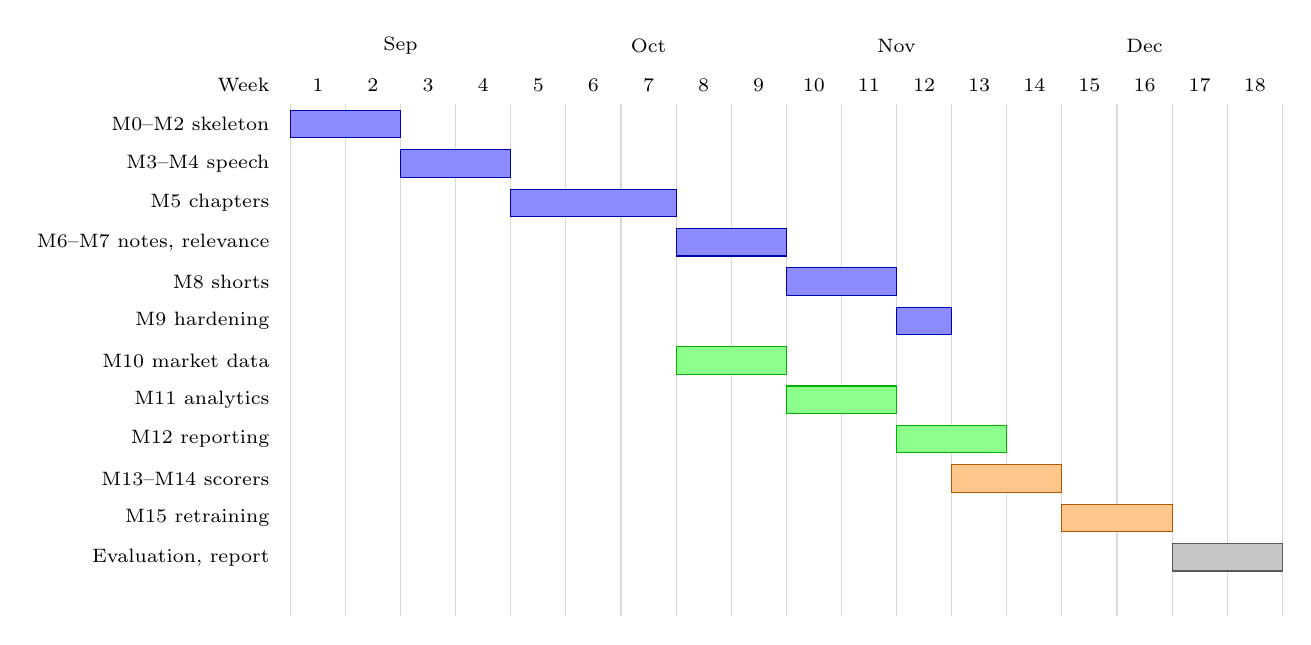
\begin{tikzpicture}[x=0.7cm, y=0.5cm]
  % week grid
  \foreach \w in {0,...,18} { \draw[gray!30] (\w,0.5) -- (\w,-12.5); }
  \foreach \w in {1,...,18} { \node[font=\scriptsize] at (\w-0.5,1) {\w}; }
  \node[font=\scriptsize, anchor=east] at (-0.2,1) {Week};
  \node[font=\scriptsize] at (2,2) {Sep};
  \node[font=\scriptsize] at (6.5,2) {Oct};
  \node[font=\scriptsize] at (11,2) {Nov};
  \node[font=\scriptsize] at (15.5,2) {Dec};
  % rows: y / label / start week / end week / colour
  \foreach \y/\lab/\s/\e/\c in {
      0/M0--M2 skeleton/1/2/blue,
      1/M3--M4 speech/3/4/blue,
      2/M5 chapters/5/7/blue,
      3/{M6--M7 notes, relevance}/8/9/blue,
      4/M8 shorts/10/11/blue,
      5/M9 hardening/12/12/blue,
      6/M10 market data/8/9/green,
      7/M11 analytics/10/11/green,
      8/M12 reporting/12/13/green,
      9/M13--M14 scorers/13/14/orange,
      10/M15 retraining/15/16/orange,
      11/{Evaluation, report}/17/18/gray} {
    \node[font=\scriptsize, anchor=east] at (-0.2,-\y) {\lab};
    \fill[\c!45, draw=\c!70!black] (\s-1,-\y-0.35) rectangle (\e,-\y+0.35);
  }
\end{tikzpicture}}
\caption{Gantt chart of the development stage. Blue: tool suite; green: market-analysis track; orange: custom models; grey: evaluation and report.}
\label{fig:gantt}
\end{figure}

The development plan identifies three milestones as high-risk, for which iteration time is budgeted beyond the estimate: the Shorts generator (M8), whose crop quality is subjective and hard to test automatically; the Reporting API integration (M12), the newest and least documented API surface; and the relevance model training (M15), for which there is no guarantee of beating the heuristic baseline. The last risk is non-blocking by design, because the heuristic model keeps the product fully functional. The same pattern was applied to the chapter generator (M5): the trained model is only deployed if it outperforms an unsupervised baseline on validation data.

%--------------------------------------------------
\section{Brief summary of the products obtained}

\textbf{YouTube Suite platform.} A monorepo containing a FastAPI back end, an arq worker, a PostgreSQL schema managed with Alembic migrations, and an Angular single-page application, deployable on a single machine with Docker Compose for the database and the queue broker.

\textbf{Speech processing tools.} GPU transcription with word-level timestamps and SRT/WebVTT export, and speaker diarization with word-level speaker assignment and speaker-aware subtitles, both sharing a 3\,GB GPU.

\textbf{Content generation tools.} A bilingual chapter generator based on locally trained models, a show-notes generator based on a local language model, and an automatic Shorts generator driven by a relevance model.

\textbf{Market-analysis pipeline.} Scheduled collection of public data (YouTube Data API~v3 and RSS feeds) and private analytics of the operator's channel (Analytics API~v2 and Reporting API~v1).

\textbf{Custom models and training pipeline.} A relevance model, a CTR predictor and a hook-strength scorer, with a model versioning and retraining pipeline; and a reproducible chapter-model experiment (notebooks, tested library and exported model bundles).

\textbf{Documentation.} Specification, development plan, decision records and research notes that trace every design decision.

%--------------------------------------------------
\section{Brief description of the other chapters of the report}

Chapter~\ref{ch:soa} reviews the state of the art in YouTube data collection, speech recognition and diarization, topic segmentation and video chaptering, highlight detection, engagement prediction and local language models.

Chapter~\ref{ch:methods} describes the requirements, technology stack, architecture, data model and methods of each component, the model training procedures, the verification strategy and an economic evaluation of the project.

Chapter~4 presents the experimental results and quantitative evaluation of the developed tools.

Chapter~5 discusses conclusions, limitations, objective achievement and future research directions.

%--------------------------------------------------
\section{Statement on the use of generative artificial intelligence}

Generative artificial intelligence was used extensively in this project, and its use is declared here in detail. An agentic coding assistant (Claude Code, based on Anthropic's Claude models) was used under the author's direction for four tasks: (i)~implementing code and tests from the design notes of each milestone; (ii)~searching and summarising literature, datasets and technical documentation; (iii)~drafting technical documentation (specification, decision records and experiment logs); and (iv)~structuring and drafting parts of this report.

The author defined the scope, took every design decision and approved every scope change; these decisions are recorded in dated decision records. The outputs of the assistant were verified through automated tests, manual end-to-end checks on real episodes and review by the author. Factual claims produced by the assistant during research were checked against primary sources before being used; this check found and corrected several wrong or unsourced claims (for instance, about dataset sizes, GPU memory requirements and published metrics), which are documented in the project's research notes. The bibliography of this report was verified in the same way. The author remains fully responsible for the content of the project and of this report.


%==========================================================
\chapter{State of the Art}
\label{ch:soa}
%==========================================================

Large VOD platforms are driven by recommendation systems trained on massive interaction data. Covington et al.\ \cite{recommender_systems_streaming} describe YouTube's two-stage deep neural recommender (candidate generation and ranking), trained to predict expected watch time rather than clicks alone, and Gomez-Uribe and Hunt \cite{vod_bigdata} report that about 80\% of the hours streamed on Netflix come from recommendations. For creators, this means that watch time, retention and CTR are the signals that determine distribution. This chapter reviews the techniques relevant to each part of the proposed platform.

\section{YouTube Data Sources}

YouTube exposes three official APIs with different scopes \cite{yt_data_api}. The \textit{Data API~v3} provides public metadata and statistics (views, likes, comments) under a default quota of 10{,}000 units per day, where a \texttt{videos.list} call costs one unit and accepts up to 50 video identifiers, while search operations are much more restricted. Per-channel RSS feeds offer a free, quota-less list of the latest uploads. The \textit{Analytics API~v2} provides private engagement and retention metrics of a channel authorised through OAuth, including audience retention curves, but it does not return impressions or CTR. Real thumbnail impressions and CTR are only available through the \textit{Reporting API~v1}, an asynchronous bulk system in which scheduled jobs produce CSV reports with a delay.

Systematic API-based collection supports large-scale research datasets. YouNiverse \cite{ribeiro2021youniverse} gathers metadata from 136k English-speaking channels and 72.9M videos with time series of views and subscribers, and Goncalves and Ng \cite{goncalves2026trending} collected three years of trending snapshots across 104 countries. None of these datasets contains impression-level CTR, which YouTube never publishes; the only source of real CTR ground truth for this project is therefore the operator's own channel.

\section{Speech Recognition and Subtitling}

Whisper \cite{radford2023whisper} is an encoder--decoder Transformer trained with weak supervision on 680{,}000 hours of multilingual audio; it approaches human robustness across accents and noise conditions and performs language identification. Its \texttt{large-v3-turbo} variant reduces the decoder from 32 to 4 layers, trading a small loss of accuracy for a large speed-up. faster-whisper \cite{fasterwhisper} re-implements Whisper inference on the CTranslate2 engine with 8-bit quantisation, which reduces memory and makes deployment on small GPUs feasible, and provides word-level timestamps. WhisperX \cite{bain2023whisperx} improves word timestamps through forced phoneme alignment and couples ASR with diarization. Research on subtitling also explores direct speech translation that produces timed subtitles in one model \cite{papi2023subtitling}; this project focuses on same-language subtitles.

\section{Speaker Diarization}

Speaker diarization answers ``who spoke when''. pyannote.audio \cite{bredin2020pyannote} provides trainable neural building blocks (voice activity detection, speaker change detection, overlapped speech detection and speaker embeddings) combined into end-to-end pipelines. Its recent pipelines use a powerset formulation of segmentation that models overlapping speakers as a multi-class problem \cite{plaquet2023powerset}, followed by embedding clustering. Since diarization produces time turns and ASR produces timed words, a final step assigns each word to a speaker turn, typically by maximum temporal overlap \cite{bain2023whisperx}.

\section{Topic Segmentation and Video Chaptering}

\subsection*{Text segmentation}

Topic segmentation divides a text into coherent segments. TextTiling \cite{hearst1997texttiling} compares lexical similarity between adjacent blocks and places boundaries at the deepest similarity valleys; the same idea applies to dense sentence embeddings, such as Sentence-BERT \cite{reimers2019sbert} or multilingual E5 \cite{wang2024me5}. Koshorek et al.\ \cite{koshorek2018textseg} reformulated segmentation as supervised sequence labelling with a bidirectional LSTM \cite{hochreiter1997lstm} over sentence representations, showing that supervised models outperform unsupervised ones when large labelled corpora are available. Segmentation quality is traditionally measured with $P_k$ \cite{beeferman1999pk} and WindowDiff \cite{pevzner2002windowdiff}.

\subsection*{Video chaptering}

Video chaptering extends segmentation with the generation of a title for each segment. VidChapters-7M \cite{yang2023vidchapters} contains 817k user-chaptered YouTube videos with 7M chapters and Whisper transcripts, and defines the task of chapter generation, with boundary metrics (recall and precision at temporal IoU thresholds) and title metrics such as CIDEr \cite{vedantam2015cider}. Chapter-Llama \cite{ventura2025chapterllama} fine-tunes an 8-billion-parameter LLM on transcripts and frame captions and is the current state of the art on hour-long videos; it also defines distance-based boundary metrics (F1 at 3 and 5 seconds). These results set the upper bound; the question addressed here is how close a much smaller model can get on consumer hardware. Titles can be generated with multilingual sequence-to-sequence models such as mT5 \cite{xue2021mt5} or with instruction-tuned LLMs.

\section{Highlight Detection and Short-Form Clip Generation}

Video summarisation selects the most important parts of a video, either as keyframes or as short excerpts \cite{apostolidis2021survey}; highlight detection scores segments by their interest. Most methods are visual: for example, SPOT \cite{kwak2025spot} integrates a CNN encoder into a TimeSformer to combine local and global spatio-temporal features. Labels are the main bottleneck. Xiong et al.\ \cite{xiong2019lessismore} learned highlights from video duration as weak supervision, and Mr.~HiSum \cite{sul2023mrhisum} uses YouTube's ``Most replayed'' statistics, aggregated from at least 50{,}000 viewers per video, as highlight labels for 31{,}892 videos.

For podcasts, the content lies mainly in the speech, which motivates text-based approaches. The open-source tools reviewed during this project segment transcripts with TextTiling-like methods or ask an LLM to pick moments, and handle the mechanical steps (cutting, vertical reframing with person or face detection, caption burn-in) with FFmpeg. Commercial services (e.g.\ OpusClip, Klap, Vizard) offer the whole pipeline as a paid cloud product. No reviewed tool trains a dedicated model to score transcript segments, and no public dataset combines long-form talk content, transcripts and continuous relevance labels at scale.

\section{Engagement and CTR Prediction}

Engagement prediction has been approached with multimodal models that combine visual, textual and, more recently, audio features; for instance, large multimodal models have been applied to predict engagement of short videos \cite{sun2025engagement}. Image--text encoders such as SigLIP~2 \cite{tschannen2025siglip2} and text encoders such as BGE \cite{xiao2023bge} provide strong frozen representations of thumbnails and titles. Because real CTR is not public and the confounders of absolute popularity (channel size, topic, promotion) are strong, pairwise learning-to-rank objectives \cite{burges2005ranknet} are well suited to comparing candidates for the same video. For small tabular datasets, gradient-boosted trees such as LightGBM \cite{ke2017lightgbm} remain the strongest choice, and SHAP values \cite{lundberg2017shap} provide per-prediction explanations. Scoring the strength of the opening seconds (``hook'') of a clip is sparsely covered in the literature because retention data is proprietary.

\section{Generative Language Models and Local Inference}

Large language models have become the standard tool for generating text such as summaries, descriptions and titles \cite{cao2023aigc}. Most applications rely on cloud APIs, but open-weight instruction-tuned models of 2 to 9 billion parameters, quantised to 4 bits and executed with engines such as llama.cpp \cite{llamacpp}, now run on commodity CPUs with acceptable latency for offline tasks. This makes fully local pipelines possible, at the cost of lower quality than the largest models and the need to validate outputs (language, format and factuality).

\section{Conclusions}

Three conclusions guide the design. First, mature open models exist for the perceptual tasks (ASR and diarization), so the engineering effort should focus on integrating them efficiently on limited hardware. Second, for chaptering and relevance scoring, state-of-the-art results rely on large models or visual features; a lightweight text-based approach, trained on public data and always compared against an unsupervised baseline, is a reasonable goal for consumer hardware. Third, real CTR and retention labels are scarce and private, which favours ranking objectives, sample-efficient models and a feedback loop that accumulates the operator's own data over time.


%==========================================================
\chapter{Materials and Methods}
\label{ch:methods}
%==========================================================

This chapter describes the scope, the technology and hardware, the architecture and data model, and the methods of each component of \textit{YouTube Suite}, followed by the verification strategy and the economic evaluation.

\section{Scope and Requirements}

The platform is designed for a single operator (the podcast producer), not as a multi-tenant service, although the architecture does not prevent that evolution. Table~\ref{tab:components} lists the v1 components and whether each one relies on an external pretrained tool or on a custom model.

\begin{table}[H]
\centering
\caption{Components of YouTube Suite v1.}
\label{tab:components}
\small
\begin{tabular}{@{}p{4.2cm}p{6.6cm}l@{}}
\toprule
\textbf{Component} & \textbf{Output} & \textbf{Approach} \\
\midrule
Transcription & Segments and words with timestamps; SRT/WebVTT & External (faster-whisper) \\
Speaker diarization & Speaker label per word and segment & External (pyannote.audio) \\
Chapter generator & Ordered chapters (start, title) & Custom (trained) \\
Show-notes generator & Titles, description, tags, summary & External (local LLM) \\
Relevance model & Relevance score per time window & Custom \\
Shorts generator & Vertical clips with optional captions & Algorithmic + detection \\
CTR predictor & Relative score of title/thumbnail candidates & Custom \\
Hook-strength scorer & Score of a clip's opening seconds & Custom \\
Market analysis & Public and private performance data & API integration \\
\bottomrule
\end{tabular}
\end{table}

The following were explicitly left out of scope for v1: thumbnail candidate extraction, multimodal (audio/visual) input to the relevance and hook models, multi-object tracking for cropping, retention drop-off prediction, a learned clip-boundary refiner, translation, multi-tenant channel connection, and automatic publication of metadata to YouTube.

\section{Technology Stack and Hardware}

\subsection*{Software}

\begin{itemize}
\item \textbf{FastAPI} \cite{fastapi_ref} for the REST API, chosen for its native asynchronous support, Pydantic validation and automatic OpenAPI documentation.
\item \textbf{PostgreSQL} as the single source of truth for platform and market data, accessed through \textbf{SQLAlchemy~2.0} \cite{sqlalchemy_ref} in asynchronous mode, with \textbf{Alembic} migrations. Enumerated columns are stored as \texttt{TEXT} with \texttt{CHECK} constraints instead of native enumerations, so that new tool types can be added with a trivial migration.
\item \textbf{arq} \cite{arq_ref} over \textbf{Redis} as the job queue. It was preferred to Celery and RQ because its tasks are native \texttt{asyncio} coroutines, which fit the asynchronous database layer without a second synchronous engine, and because it adds a single lightweight service.
\item \textbf{Angular} \cite{angular_ref} with standalone components and signals for the front end.
\item \textbf{PyTorch} \cite{paszke2019pytorch} (CUDA~12.6 build, the last line with kernels for the Pascal architecture), \textbf{faster-whisper}, \textbf{pyannote.audio}, \textbf{sentence-transformers}, \textbf{Hugging Face Transformers}, \textbf{llama.cpp} \cite{llamacpp}, \textbf{LightGBM} and \textbf{FFmpeg} for the model and media layers.
\item \textbf{Docker Compose} \cite{merkel2014docker} for PostgreSQL and Redis; \textbf{pytest} and \textbf{Vitest} for testing.
\end{itemize}

\subsection*{Hardware}

The production target is the operator's own computer: an AMD Ryzen~5~2600X CPU (6 cores, 12 threads), 16\,GB of RAM, and an NVIDIA GTX~1060 GPU with 3\,GB of memory (Pascal architecture, compute capability~6.1). This GPU supports only 8-bit integer and 32-bit floating-point inference in CTranslate2 and has no fast half-precision arithmetic, and about 0.5\,GB of its memory is used by the desktop. These constraints shape many of the decisions below: GPU memory is treated as a budget shared by the models, and every model that does not fit or does not need the GPU runs on the CPU.

\section{System Architecture}

Figure~\ref{fig:architecture} shows the architecture. The Angular client talks only to the REST API. Every AI tool is executed as a job: the API creates a row in the \texttt{jobs} table and enqueues its identifier in Redis; a separate worker process consumes it and updates the job's state and results in PostgreSQL. Media files (uploaded videos, extracted audio and exported clips) are stored behind a \texttt{StorageBackend} interface (\texttt{save}, \texttt{get}, \texttt{delete}) implemented on the local file system, so that a future move to S3-compatible storage requires no change in the calling code; the database stores only backend-relative keys.

\begin{figure}[H]
\centering
\resizebox{\textwidth}{!}{%
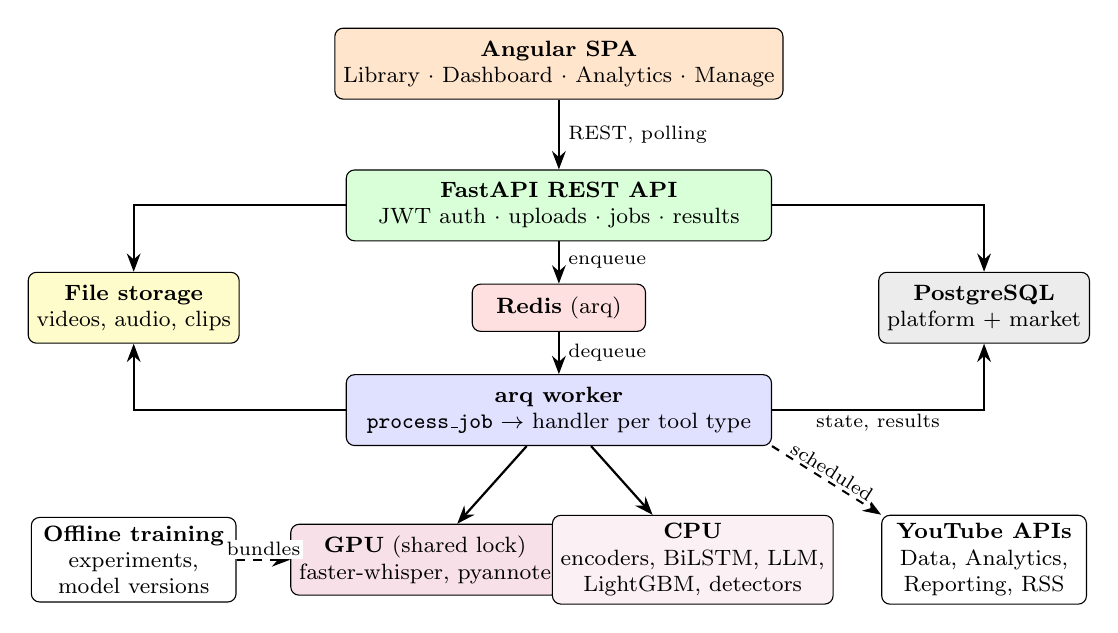
\begin{tikzpicture}[
    box/.style={draw, rounded corners=3pt, align=center, font=\footnotesize,
                minimum height=0.9cm, inner sep=3pt},
    arr/.style={-Stealth, thick},
    darr/.style={-Stealth, thick, dashed},
    lab/.style={font=\scriptsize, fill=white, inner sep=1pt}
]
\node[box, fill=orange!20, minimum width=5.4cm] (fe) at (0,5.4)
  {\textbf{Angular SPA}\\Library $\cdot$ Dashboard $\cdot$ Analytics $\cdot$ Manage};
\node[box, fill=green!15, minimum width=5.4cm] (api) at (0,3.6)
  {\textbf{FastAPI REST API}\\JWT auth $\cdot$ uploads $\cdot$ jobs $\cdot$ results};
\node[box, fill=red!12, minimum width=2.2cm, minimum height=0.6cm] (redis) at (0,2.3)
  {\textbf{Redis} (arq)};
\node[box, fill=blue!12, minimum width=5.4cm] (worker) at (0,1.0)
  {\textbf{arq worker}\\\texttt{process\_job} $\rightarrow$ handler per tool type};
\node[box, fill=gray!15, minimum width=2.6cm] (pg) at (5.4,2.3)
  {\textbf{PostgreSQL}\\platform + market};
\node[box, fill=yellow!20, minimum width=2.6cm] (store) at (-5.4,2.3)
  {\textbf{File storage}\\videos, audio, clips};
\node[box, fill=purple!12, minimum width=3.0cm] (gpu) at (-1.7,-0.9)
  {\textbf{GPU} (shared lock)\\faster-whisper, pyannote};
\node[box, fill=purple!6, minimum width=3.0cm] (cpu) at (1.7,-0.9)
  {\textbf{CPU}\\encoders, BiLSTM, LLM,\\LightGBM, detectors};
\node[box, fill=white, minimum width=2.6cm] (yt) at (5.4,-0.9)
  {\textbf{YouTube APIs}\\Data, Analytics,\\Reporting, RSS};
\node[box, fill=white, minimum width=2.6cm] (train) at (-5.4,-0.9)
  {\textbf{Offline training}\\experiments,\\model versions};

\draw[arr] (fe) -- node[lab, right=2pt] {REST, polling} (api);
\draw[arr] (api) -- node[lab, right=2pt] {enqueue} (redis);
\draw[arr] (redis) -- node[lab, right=2pt] {dequeue} (worker);
\draw[arr] (api.east) -| (pg.north);
\draw[arr] (worker.east) -| node[lab, pos=0.25, below] {state, results} (pg.south);
\draw[arr] (api.west) -| (store.north);
\draw[arr] (worker.west) -| (store.south);
\draw[arr] (worker) -- (gpu);
\draw[arr] (worker) -- (cpu);
\draw[darr] (worker.south east) -- node[lab, sloped, above] {scheduled} (yt.north west);
\draw[darr] (train) -- node[lab, above] {bundles} (gpu);
\end{tikzpicture}}
\caption{Architecture of YouTube Suite. Solid arrows: request and job flow; dashed arrows: scheduled market collection and deployment of trained models.}
\label{fig:architecture}
\end{figure}

\subsection*{Job pipeline}

All tools share a single execution path (Figure~\ref{fig:jobs}). \texttt{POST /uploads/\{id\}/jobs} creates a job with a \texttt{tool\_type} and enqueues the generic task \texttt{process\_job(job\_id)}. The worker marks the job as \textit{running}, looks up the handler registered for its tool type, runs it with a database session, and marks the job as \textit{succeeded}, or as \textit{failed} with the error message if an exception is raised. Adding a tool only requires registering a new handler; neither the queue, the state machine nor the front end change. Handlers replace their outputs within a single transaction, so re-running a tool is idempotent and readers never see a partial result. Tools that depend on the transcript fail fast with an explicit message when no successful transcription exists. The front end polls job states every three seconds; websockets were not needed at this scale.

\begin{figure}[H]
\centering
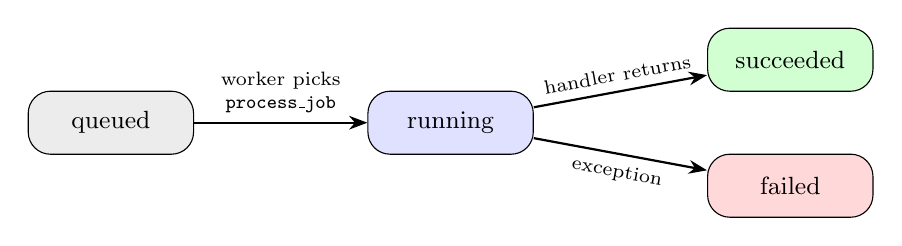
\begin{tikzpicture}[
    st/.style={draw, rounded corners=8pt, minimum width=2.1cm, minimum height=0.8cm, font=\small},
    arr/.style={-Stealth, thick},
    lab/.style={font=\scriptsize, align=center}
]
\node[st, fill=gray!15] (q) {queued};
\node[st, fill=blue!12, right=2.2cm of q] (r) {running};
\node[st, fill=green!18, right=2.2cm of r, yshift=0.8cm] (s) {succeeded};
\node[st, fill=red!15, right=2.2cm of r, yshift=-0.8cm] (f) {failed};
\draw[arr] (q) -- node[lab, above] {worker picks\\\texttt{process\_job}} (r);
\draw[arr] (r) -- node[lab, above, sloped] {handler returns} (s);
\draw[arr] (r) -- node[lab, below, sloped] {exception} (f);
\end{tikzpicture}
\caption{State machine of a job. The same path is shared by all tool types.}
\label{fig:jobs}
\end{figure}

\subsection*{GPU resource management}

Whisper and pyannote are kept resident on the GPU as lazily loaded per-process singletons, and a shared lock ensures that only one GPU inference runs at a time, so that their memory peaks never add up. Measured peaks on a full 64-minute episode were 2016\,MiB of total GPU memory during transcription and 2398\,MiB during diarization with Whisper resident, out of 3072\,MiB. The diarization pipeline releases PyTorch's cached memory after every run; without this step, memory reserved by the start-up health check caused an out-of-memory error in the following transcription, a failure that was found during manual verification and is covered by a regression test. All other models (chapter models, language models, scorers and detectors) run on the CPU and do not take the GPU lock.

\subsection*{Security}

Authentication uses the OAuth2 password flow with JWT access tokens (HS256, 12-hour expiry) and bcrypt password hashes. As the platform has a single operator, the user is created by a command-line tool and there is no public registration. Video previews are streamed with HTTP range requests; because a browser \texttt{<video>} element cannot send an authorisation header, this single endpoint also accepts the token as a query parameter, a trade-off accepted for a single-operator tool.

\section{Data Model}

The database is organised into platform data and market data (Table~\ref{tab:datamodel}). Tool outputs are stored as rows linked to the upload and deleted in cascade with it; outputs produced by custom models reference the model version that produced them, which makes every prediction traceable and allows comparing versions.

\begin{table}[H]
\centering
\caption{Main tables of the data model.}
\label{tab:datamodel}
\small
\begin{tabular}{@{}p{4.3cm}p{9.2cm}@{}}
\toprule
\textbf{Table} & \textbf{Content} \\
\midrule
\multicolumn{2}{@{}l}{\textit{Platform data}} \\
\texttt{users} & Single operator account (e-mail, password hash). \\
\texttt{uploads} & Original file name, storage key, duration, extracted-audio key, status. \\
\texttt{jobs} & Tool type, state, progress, start and end times, error message. \\
\texttt{transcript\_segments} & Segment index, start/end, text, confidence proxies, speaker label. \\
\texttt{transcript\_words} & Word, start/end, probability, speaker label (linked to its segment). \\
\texttt{chapters} & Order, start time, title and version of the models that produced it. \\
\texttt{relevance\_scores} & Window start/end, score in $[0,1]$, model version. \\
\texttt{clips} & Source span, aspect ratio, caption flag, file key, smoothed crop track (JSONB). \\
\texttt{show\_notes\_drafts} & Title suggestions, description, tags, summary, language model used. \\
\texttt{ctr\_predictions} & Candidate title and thumbnail, predicted relative score, model version. \\
\texttt{hook\_scores} & Clip, score, engineered feature vector (JSONB), model version. \\
\texttt{model\_versions} & Model name, architecture, training data reference, metrics, artefact, live flag. \\
\midrule
\multicolumn{2}{@{}l}{\textit{Market data}} \\
\texttt{market\_channels} & Curated list of public podcast channels. \\
\texttt{market\_video\_snapshots} & Daily snapshot of public metadata and statistics per video. \\
\texttt{analytics\_snapshots} & Daily engagement of the operator's own videos. \\
\texttt{analytics\_retention\_curve} & Audience retention per elapsed-time bucket. \\
\texttt{analytics\_reach\_snapshots} & Real thumbnail impressions and CTR (Reporting API). \\
\texttt{reporting\_jobs} & State of the asynchronous Reporting API jobs. \\
\texttt{oauth\_credentials} & Encrypted OAuth tokens of the connected channel. \\
\bottomrule
\end{tabular}
\end{table}

Market snapshots are stored as time series (one row per video and day) instead of being overwritten, which enables the analysis of growth curves. Deprecated or unavailable fields (\texttt{favoriteCount}, \texttt{dislikeCount}) are deliberately excluded.

\section{Transcription and Subtitles}

Transcription is the root of the tool graph (Figure~\ref{fig:speech}). FFmpeg extracts the audio track as 16\,kHz mono WAV, which is persisted in storage because diarization reuses it. faster-whisper runs the \texttt{large-v3-turbo} model with 8-bit quantisation on the GPU, word-level timestamps, beam size~5, voice activity detection to avoid hallucinations over silence and music, and automatic language detection. A measured spike on the target GPU gave about 14.7$\times$ real time on a 10-minute clip with 1.55\,GB of model memory; the CPU remains a configuration-only fallback. Segments and words are replaced in one transaction.

SRT and WebVTT files are generated on demand from the stored rows instead of being cached, since generation is linear in the number of segments and a cache would have to be invalidated after every re-transcription or diarization. The formatter rounds timestamps to whole milliseconds, clamps invalid intervals, removes blank lines that would end a cue early and escapes WebVTT control characters.

\begin{figure}[H]
\centering
\resizebox{\textwidth}{!}{%
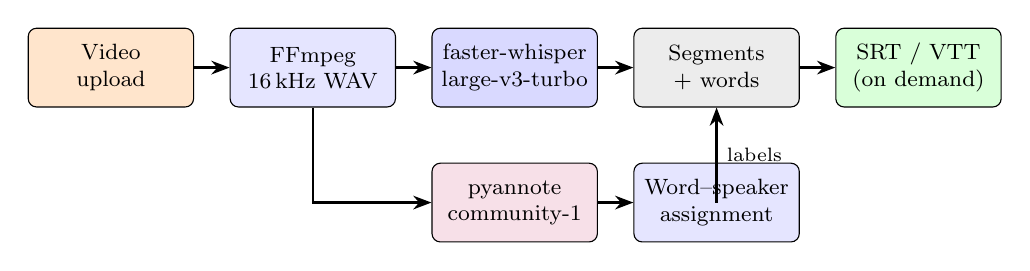
\begin{tikzpicture}[
    node distance=0.45cm,
    b/.style={draw, rounded corners=3pt, align=center, font=\footnotesize,
              minimum height=1.0cm, minimum width=2.1cm, fill=#1},
    arr/.style={-Stealth, thick}
]
\node[b=orange!20] (v) {Video\\upload};
\node[b=blue!10, right=of v] (a) {FFmpeg\\16\,kHz WAV};
\node[b=blue!15, right=of a] (w) {faster-whisper\\large-v3-turbo};
\node[b=gray!15, right=of w] (t) {Segments\\+ words};
\node[b=green!15, right=of t] (s) {SRT / VTT\\(on demand)};
\node[b=purple!12, below=0.7cm of w] (p) {pyannote\\community-1};
\node[b=blue!10, right=of p] (as) {Word--speaker\\assignment};
\draw[arr] (v) -- (a);
\draw[arr] (a) -- (w);
\draw[arr] (w) -- (t);
\draw[arr] (t) -- (s);
\draw[arr] (a) |- (p);
\draw[arr] (p) -- (as);
\draw[arr] (as) -| node[font=\scriptsize, pos=0.75, right] {labels} (t);
\end{tikzpicture}}
\caption{Speech processing: transcription (top) and diarization (bottom) share the extracted audio and the transcript rows.}
\label{fig:speech}
\end{figure}

\section{Speaker Diarization}

Diarization uses pyannote.audio~4 with the \texttt{speaker-diarization-community-1} pipeline \cite{bredin2020pyannote}, keeping its overlap-free (\textit{exclusive}) output so that at most one speaker is active at any instant. A spike showed that the CPU runs below real time, whereas the GPU reaches about 17$\times$ real time; reducing the embedding batch size to~8 lets pyannote coexist with Whisper on the GPU without loss of speed. WhisperX was not used because its dependency constraints conflict with the other libraries, so the word--speaker assignment was reimplemented as pure, unit-tested functions:
\begin{itemize}
\item each word takes the speaker turn with the largest temporal overlap, or the nearest turn if it falls in a gap; words without timestamps remain unlabelled;
\item each segment takes the majority speaker of its words, with ties broken by the first labelled word;
\item labels are renamed by order of first appearance, and turns are searched by bisection to avoid a quadratic cost.
\end{itemize}

Because a failure to accept the model's licence or an invalid token makes the pipeline fail silently, the worker runs a health check at start-up on a bundled synthetic two-speaker clip and requires a non-empty output with at least two speakers. If it fails, only diarization jobs are disabled, with the reason shown in the interface. Subtitles include speakers when available (\texttt{[SPEAKER\_00]} prefixes in SRT and voice spans in WebVTT). Because Whisper segments often contain short interjections of another speaker, a segment whose word labels change speaker is split into one cue per speaker run; runs shorter than two words are merged into a neighbour to avoid cues produced by a single mislabelled word.

\section{Chapter Generation}

Chapters are generated with two models trained locally for this project, a boundary model and a title model, developed as a documented experiment. The initial specification proposed an external LLM API followed by a lexical realignment of the returned boundaries; it was replaced to keep processing local and to predict boundaries directly on real transcript units, which makes realignment unnecessary. Figure~\ref{fig:chapters} summarises the pipeline.

\begin{figure}[H]
\centering
\resizebox{\textwidth}{!}{%
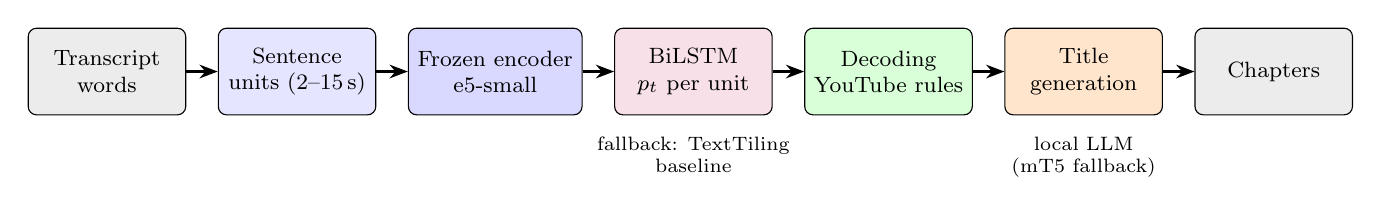
\begin{tikzpicture}[
    node distance=0.4cm,
    b/.style={draw, rounded corners=3pt, align=center, font=\footnotesize,
              minimum height=1.1cm, minimum width=2.0cm, fill=#1},
    arr/.style={-Stealth, thick}
]
\node[b=gray!15] (t) {Transcript\\words};
\node[b=blue!10, right=of t] (u) {Sentence\\units (2--15\,s)};
\node[b=blue!15, right=of u] (e) {Frozen encoder\\e5-small};
\node[b=purple!12, right=of e] (l) {BiLSTM\\$p_t$ per unit};
\node[b=green!15, right=of l] (d) {Decoding\\YouTube rules};
\node[b=orange!20, right=of d] (ti) {Title\\generation};
\node[b=gray!15, right=of ti] (c) {Chapters};
\draw[arr] (t) -- (u);
\draw[arr] (u) -- (e);
\draw[arr] (e) -- (l);
\draw[arr] (l) -- (d);
\draw[arr] (d) -- (ti);
\draw[arr] (ti) -- (c);
\node[font=\scriptsize, below=0.15cm of l, align=center] {fallback: TextTiling\\baseline};
\node[font=\scriptsize, below=0.15cm of ti, align=center] {local LLM\\(mT5 fallback)};
\end{tikzpicture}}
\caption{Chapter generation pipeline. All inference runs on the CPU.}
\label{fig:chapters}
\end{figure}

\subsection*{Training data}

The models are trained on VidChapters-7M \cite{yang2023vidchapters}, obtained from the JSON mirror published with Chapter-Llama \cite{ventura2025chapterllama}. The original transcript file is a single 19\,GB pickle that does not fit in memory, so the chapter file (2\,GB) and the transcript file (22\,GB) are streamed and only the selected videos are kept. Videos are selected with a duration between 15 and 120 minutes, at least three chapters of at least 10 seconds, and a usable transcript. The language is identified on the transcript rather than on the titles, because title-based identification proved unreliable in both directions (titles in Spanish over English speech and vice versa). The result is about 9{,}000 English training videos with the official validation and test splits, and only 207 videos with Spanish speech, split by channel into training, validation and a Spanish-only test set used to measure cross-lingual transfer.

\subsection*{Text units}

VidChapters transcripts are split into sentences of about 5 seconds, whereas the platform's Whisper segments have a median of 0.8 seconds. To avoid a train--inference mismatch, both sides are normalised to the same unit before encoding: sentences rebuilt from word timestamps and punctuation, with durations between 2 and 15 seconds. This unit was chosen over fixed time blocks because it has the highest boundary ceiling (the best score achievable after snapping reference boundaries to unit starts). The same function is used in the experiment and in the back end, and a test fails if both copies diverge.

\subsection*{Boundary model}

Each unit is encoded with the frozen multilingual encoder \texttt{multilingual-e5-small} \cite{wang2024me5} (118M parameters), chosen over an equivalent MiniLM model for its licence and similar accuracy, and over larger encoders because it encodes a one-hour episode in about 7 seconds on the CPU. A linear projection of the embeddings, concatenated with two side features (the unit's relative position in the episode and its cosine similarity to the previous unit), feeds a bidirectional LSTM \cite{hochreiter1997lstm, koshorek2018textseg} that outputs the probability $p_t$ that a chapter starts at unit $t$. Since boundaries are rare (about one every 40 units), training uses a class-weighted binary cross-entropy with softened targets $\tilde y_t$ around each reference boundary:
\begin{equation}
\mathcal{L} = -\frac{1}{T}\sum_{t=1}^{T}\Big[w_{+}\,\tilde y_t\log p_t + (1-\tilde y_t)\log(1-p_t)\Big],
\label{eq:bce}
\end{equation}
where $w_{+}$ is the positive-class weight. Checkpoints are selected by the validation F1 at 5 seconds after decoding, i.e.\ on the same output that is deployed.

\subsection*{Decoding}

YouTube's rules and the desired granularity (few, broad chapters) are applied at decoding time rather than learnt: peaks of $p_t$ are selected with a minimum chapter length of 60 seconds and a target of about six chapters per hour; the first chapter is forced to 0:00, at least three chapters are produced and every chapter lasts at least 10 seconds. Every boundary lands on a real transcript timestamp.

\subsection*{Baseline and deployment rule}

An unsupervised TextTiling-style baseline \cite{hearst1997texttiling} computes the cosine dissimilarity between adjacent windows of the same unit embeddings and uses the same decoding. It requires no training and serves both as the evaluation reference and as the production fallback: the trained model is deployed only if it outperforms the baseline on validation F1 at 5 seconds.

\subsection*{Title model}

Titles are generated for each predicted chapter from its transcript text. Two approaches were developed. The first fine-tunes \texttt{mt5-small} \cite{xue2021mt5} on pairs of chapter text and user title; full fine-tuning did not fit in 3\,GB even with batch size~1, so the shared embedding matrix and the output layer (256M of 300M parameters) were frozen, and Adafactor \cite{shazeer2018adafactor} with gradient checkpointing was used; the few Spanish pairs were oversampled. Because the resulting Spanish titles were not usable on real episodes and no more Spanish training data exists, the second approach uses a pretrained open-weight instruction LLM executed locally with llama.cpp \cite{llamacpp} (4-bit GGUF quantisation, CPU only). Several models of 2 to 9 billion parameters were compared with the same prompt, which asks for one short title in the language of the episode without invented names. Outputs are post-processed (removal of quotes and prefixes, collapse of repeated n-grams, length cap, language check), and a title that fails validation is retried once and then generated with mT5. The model was selected by a blind review of titles among the candidates that passed three gates: at least 95\% language accuracy in Spanish, CIDEr not far below mT5, and at most 15 minutes of CPU time for a one-hour episode.
% TODO: name the LLM selected in experiment 06 once the blind review is done.

\subsection*{Evaluation protocol}

Boundaries are evaluated with the distance-based F1 at 3 and 5 seconds and the temporal-IoU-averaged F1 of Chapter-Llama \cite{ventura2025chapterllama}, together with $P_k$ \cite{beeferman1999pk}, WindowDiff \cite{pevzner2002windowdiff} and the error in the number of chapters. The metric implementation was cross-checked against the Chapter-Llama code on synthetic data, with identical results. Each metric is reported in two settings: the \textit{product} setting, with the deployed granularity, and an \textit{oracle} setting in which the number of chapters is known, since creators tend to annotate more chapters than the product produces. Titles are evaluated with BLEU \cite{papineni2002bleu} and CIDEr \cite{vedantam2015cider} on reference boundaries, language accuracy and repetition rate, and by manual review. Model selection uses validation data only; the test sets are evaluated once.

\subsection*{Integration}

The experiment exports a versioned bundle (encoder, BiLSTM weights, title model, unit and decoding configuration, and metrics). The \texttt{chapters} handler loads it lazily on the CPU and stores each chapter with a \texttt{model\_version} string. The interface lists the chapters and copies them in YouTube's \texttt{00:00 Title} format.

\section{Show-Notes Generation}

The show-notes generator produces a structured draft with title suggestions, a description, tags and a summary. It uses the same local runtime as the chapter titles (llama.cpp on the CPU) to keep the whole platform local. The prompt combines the transcript and, when available, the chapters; transcripts that exceed the model's context are first summarised by parts and the partial summaries are then combined. The model is asked for JSON output, which is validated against a schema; malformed responses are repaired or regenerated a limited number of times before the job fails. The draft is stored together with the model identifier for reproducibility and can be edited in the interface. Publication to YouTube remains manual.

\section{Relevance Model}

The relevance model assigns each moment of the episode a score in $[0,1]$ that reflects how interesting it is as standalone content; it drives the Shorts generator. The transcript is re-chunked into sliding windows of 10 to 20 seconds with 50\% overlap, built from word timestamps and independent of Whisper's segment boundaries.

\textbf{Bootstrap version (v0).} Since no labelled data exists at the start, the first version combines heuristic rules (anchoring to the episode's topics, question--answer pairs, density of speaker changes and ratio of filler words) with a zero-shot score from the local LLM, which rates each window from 0 to 100. Its outputs are stored with a heuristic model version.

\textbf{Trained version.} Each window is embedded with a frozen \texttt{bge-base-en-v1.5} encoder \cite{xiao2023bge}, and a BiLSTM over the sequence of window embeddings followed by a small MLP with a sigmoid output produces the score. Long episodes are processed in overlapping super-chunks whose overlapping scores are averaged. The model is trained by distillation from the noisy pseudo-labels $y_t$ of the bootstrap version, using the Huber loss $\ell_\delta$, which is robust to label noise, plus a temporal smoothness term, since relevance is autocorrelated in time:
\begin{equation}
\mathcal{L} = \frac{1}{T}\sum_{t=1}^{T}\ell_\delta\big(s_t, y_t\big) + \lambda\sum_{t=2}^{T}\big(s_t - s_{t-1}\big)^2 .
\label{eq:relevance}
\end{equation}
As retention data from the operator's channel accumulates, pseudo-labels are progressively replaced by labels derived from audience retention, following the idea of Mr.~HiSum \cite{sul2023mrhisum}. A recurrent head over frozen embeddings was preferred to a Transformer because it has far fewer parameters and trains stably on small, noisy datasets.

\section{Shorts Generator}

The Shorts generator turns the relevance curve into vertical clips without human intervention (Figure~\ref{fig:shorts}). Its steps are implemented as separately testable units:
\begin{enumerate}
\item \textbf{Peak finding}: local maxima of the relevance curve with a minimum prominence.
\item \textbf{Boundary expansion}: from each peak, the span grows while the score stays above a fraction (about 70\%) of the peak height, up to a maximum duration.
\item \textbf{Sentence snapping}: start and end are moved to the nearest sentence boundary, so that cuts never fall mid-sentence.
\item \textbf{Constraints}: candidates below the minimum duration are discarded, longer ones are truncated, and overlapping candidates are merged.
\item \textbf{Cut and reframe}: FFmpeg cuts each span; a lightweight person/face detector, adapted from open-source reframing tools, is run on sampled frames, the bounding-box track is smoothed over time to avoid jitter, and a crop window with the selected aspect ratio (9:16 by default) is applied during re-encoding.
\item \textbf{Captions}: optionally, a subtitle slice of the clip's time range is generated from the stored transcript and burned in within the same encoding pass.
\end{enumerate}
Each clip is stored with its span, aspect ratio, crop track and a reference to the relevance windows it came from, so that its performance can later be traced back to its source segment.

\begin{figure}[H]
\centering
\resizebox{\textwidth}{!}{%
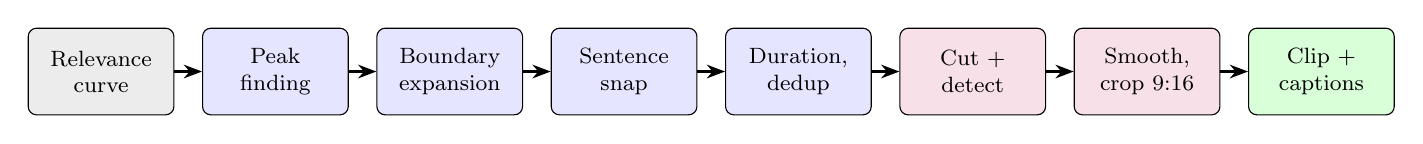
\begin{tikzpicture}[
    node distance=0.35cm,
    b/.style={draw, rounded corners=3pt, align=center, font=\footnotesize,
              minimum height=1.1cm, minimum width=1.85cm, fill=#1},
    arr/.style={-Stealth, thick}
]
\node[b=gray!15] (r) {Relevance\\curve};
\node[b=blue!10, right=of r] (p) {Peak\\finding};
\node[b=blue!10, right=of p] (x) {Boundary\\expansion};
\node[b=blue!10, right=of x] (s) {Sentence\\snap};
\node[b=blue!10, right=of s] (d) {Duration,\\dedup};
\node[b=purple!12, right=of d] (c) {Cut +\\detect};
\node[b=purple!12, right=of c] (m) {Smooth,\\crop 9:16};
\node[b=green!15, right=of m] (o) {Clip +\\captions};
\draw[arr] (r) -- (p);
\draw[arr] (p) -- (x);
\draw[arr] (x) -- (s);
\draw[arr] (s) -- (d);
\draw[arr] (d) -- (c);
\draw[arr] (c) -- (m);
\draw[arr] (m) -- (o);
\end{tikzpicture}}
\caption{Shorts generation pipeline: selection of spans (blue) and video processing (purple).}
\label{fig:shorts}
\end{figure}

\section{Market-Analysis Pipeline}

The market-analysis pipeline collects the data that the custom models need (Figure~\ref{fig:market}). It runs as scheduled jobs in the same worker and consists of three integrations with different patterns:

\textbf{Public data (Data API~v3).} For each channel in a curated list of podcast channels, the free RSS feed is checked frequently to discover new uploads, and a daily pull retrieves metadata and statistics with \texttt{videos.list}, batching 50 identifiers per call, the cheapest operation of the quota. Search calls are reserved for occasional discovery. ISO~8601 durations are parsed to seconds and statistics are cast from strings.

\textbf{Private engagement (Analytics API~v2).} A single platform-level OAuth connection with read-only scope retrieves daily per-video engagement and audience retention curves. The API allows only one video per retention request, so retention is pulled in a per-video loop. Token refresh and revocation are handled explicitly, because they are a classic source of silent failures.

\textbf{Real CTR (Reporting API~v1).} Impressions and CTR are only available through reporting jobs (\texttt{channel\_reach\_basic\_a1}). The pipeline creates the job once, polls it periodically, downloads and parses the CSV reports when they become available, and tolerates the reporting delay inherent to this API.

\begin{figure}[H]
\centering
\resizebox{0.95\textwidth}{!}{%
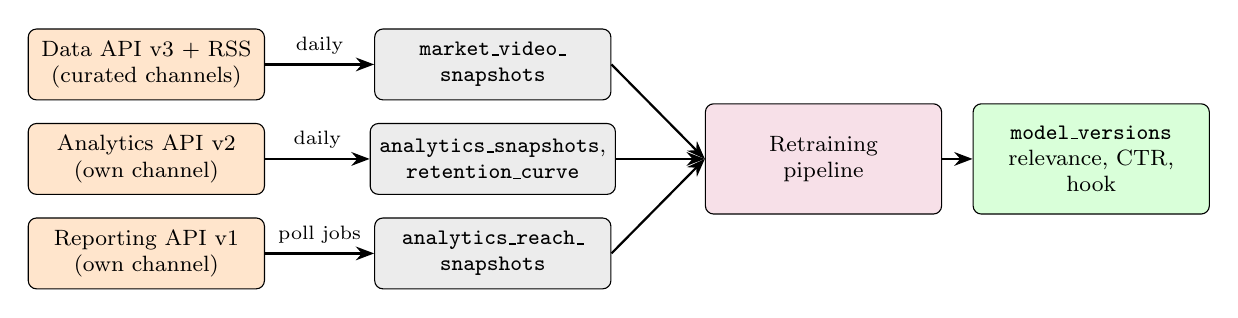
\begin{tikzpicture}[
    b/.style={draw, rounded corners=3pt, align=center, font=\footnotesize,
              minimum height=0.9cm, minimum width=3.0cm, fill=#1},
    arr/.style={-Stealth, thick}
]
\node[b=orange!20] (d) at (0,2.4) {Data API v3 + RSS\\(curated channels)};
\node[b=orange!20] (a) at (0,1.2) {Analytics API v2\\(own channel)};
\node[b=orange!20] (r) at (0,0) {Reporting API v1\\(own channel)};
\node[b=gray!15] (td) at (4.4,2.4) {\texttt{market\_video\_}\\\texttt{snapshots}};
\node[b=gray!15] (ta) at (4.4,1.2) {\texttt{analytics\_snapshots},\\\texttt{retention\_curve}};
\node[b=gray!15] (tr) at (4.4,0) {\texttt{analytics\_reach\_}\\\texttt{snapshots}};
\node[b=purple!12, minimum height=1.4cm] (tr2) at (8.6,1.2) {Retraining\\pipeline};
\node[b=green!15, minimum height=1.4cm] (mv) at (12.0,1.2) {\texttt{model\_versions}\\relevance, CTR,\\hook};
\draw[arr] (d) -- node[font=\scriptsize, above] {daily} (td);
\draw[arr] (a) -- node[font=\scriptsize, above] {daily} (ta);
\draw[arr] (r) -- node[font=\scriptsize, above] {poll jobs} (tr);
\draw[arr] (td.east) -- (tr2.west);
\draw[arr] (ta.east) -- (tr2.west);
\draw[arr] (tr.east) -- (tr2.west);
\draw[arr] (tr2) -- (mv);
\end{tikzpicture}}
\caption{Market-analysis data sources and the feedback loop into the custom models.}
\label{fig:market}
\end{figure}

\section{CTR Predictor and Hook-Strength Scorer}

\subsection*{CTR predictor}

The CTR predictor compares candidate title and thumbnail pairs for the same episode. The initial version is a weighted combination of engineered features: title length and word count, presence of numbers and question marks, number and size of faces in the thumbnail, and area covered by text (obtained with OCR). The trained version embeds the thumbnail with a frozen SigLIP~2 image encoder \cite{tschannen2025siglip2} and the title with the frozen BGE text encoder, projects both to a 256-dimensional space, concatenates them with the engineered features and applies a fusion MLP that outputs a scalar score $f(x)$. It is trained with a pairwise ranking loss \cite{burges2005ranknet} over pairs $(i,j)$ of the same video in which $i$ obtained a higher real CTR than $j$:
\begin{equation}
\mathcal{L} = \sum_{(i,j)} \log\!\Big(1 + e^{-\left(f(x_i) - f(x_j)\right)}\Big).
\label{eq:ranknet}
\end{equation}
The ranking formulation was preferred to regression for four reasons: real CTR is scarce and noisy; comparing candidates of the same video cancels confounders such as channel size or topic; $N$ candidates yield $\mathcal{O}(N^2)$ training pairs; and ranking is exactly what the product needs. Scores are therefore relative, not calibrated CTR percentages.

\subsection*{Hook-strength scorer}

The hook scorer evaluates the first 5 to 15 seconds of each clip. It extracts about fifteen engineered features from the opening transcript: length and readability, questions and exclamations (and whether the first sentence is a question), superlatives and numbers, direct address and imperatives, curiosity-gap connectives, named-entity density, an emotion score used as an arousal proxy, speaking pace from word timestamps, and overlap with the episode title. The initial version combines them with heuristic weights; the trained version uses LightGBM \cite{ke2017lightgbm} with a pairwise ranking objective, the most sample-efficient option for small tabular data. The feature vector is stored with each score, so SHAP values \cite{lundberg2017shap} can explain why a hook is weak (e.g.\ ``no question in the first sentence'').

\section{Model Versioning and Retraining}

Every trained model is registered in \texttt{model\_versions} with its architecture, training data reference, validation metrics, artefact location and a flag that marks the version used for inference. A periodic retraining job builds training sets from the accumulated market data and the stored clips, trains new versions and evaluates them on held-out data. A new version is only marked as live when it outperforms the current one; otherwise the previous version, ultimately the heuristic one, remains in production. This rollback-by-default policy makes the training loop non-blocking: the product is fully usable even if a training round fails to improve the model.

\section{User Interface}

The Angular interface has four authenticated pages: a \textit{Library} of uploaded episodes, a \textit{Dashboard} with key indicators, an \textit{Analytics} page with market and channel data, and a \textit{Manage} page where each episode can be previewed and every tool can be run, monitored and inspected. The \textit{Manage} page shows the state of each job (with the failure reason as a tooltip), allows downloading subtitles, lists the chapters with a copy-to-YouTube action, and displays show notes, clips and scores. Tools that require a transcript are disabled until one exists.

\section{Verification Strategy}

Verification was part of every milestone and combined several levels:
\begin{itemize}
\item \textbf{Unit tests} for pure logic: subtitle formatting, speaker assignment, text units, decoding rules, metrics, windowing, peak finding and feature extractors.
\item \textbf{Handler tests} with mocked models and real FFmpeg, checking persistence, idempotent re-runs and explicit failures.
\item \textbf{Integration tests} running real models on small fixtures with licence-compatible audio (LibriSpeech, CC~BY~4.0): the transcript must reach a word error rate below 0.15 and diarization must label at least 90\% of the words correctly on a synthetic two-speaker conversation. A test that runs a real worker checks the complete chain of job states.
\item \textbf{Migration tests} (upgrade and downgrade) and \textbf{API tests} for every endpoint, including authorisation and error codes.
\item \textbf{Front-end component tests} with Vitest.
\item \textbf{Experiment tests} for the model library, including a check that the metrics match the reference implementation.
\item \textbf{Manual end-to-end checks} on a real 64-minute bilingual podcast episode, which revealed defects that automated tests had not caught (non-ASCII file names in download headers, and the GPU memory issue described above); each defect was turned into a regression test.
\end{itemize}
The complete suite is re-run at the end of every milestone as a regression check, and a dedicated hardening milestone (M9) runs the whole pipeline on several real episodes.

%--------------------------------------------------
\section{Economic Evaluation of the Project}

\subsection{Development Costs}

Table~\ref{tab:dev_costs} estimates the development effort from the milestone estimates of the development plan, at 6 productive hours per day and an hourly rate of \texteuro22, representative of a junior data scientist or developer in Spain.

\begin{table}[H]
\centering
\caption{Estimated development cost.}
\label{tab:dev_costs}
\small
\begin{tabular}{@{}lrr@{}}
\toprule
\textbf{Area} & \textbf{Hours} & \textbf{Cost (\texteuro)} \\
\midrule
Design stage (scope, research, specification, planning) & 40 & 880 \\
Back-end core, job pipeline and hardening (M0, M2, M9) & 84 & 1,848 \\
Front end (M1 and interface) & 40 & 880 \\
Speech processing (M3, M4) & 51 & 1,122 \\
Chapter models and integration (M5) & 75 & 1,650 \\
Show notes, relevance v0 and Shorts (M6--M8) & 98 & 2,156 \\
Market-analysis pipeline (M10--M12) & 105 & 2,310 \\
CTR, hook and retraining (M13--M15) & 132 & 2,904 \\
Documentation and report & 60 & 1,320 \\
\midrule
\textbf{Total} & \textbf{685} & \textbf{15,070} \\
\bottomrule
\end{tabular}
\end{table}

\subsection{Operating Costs}

Because the platform runs on hardware the operator already owns and uses no paid services, operating costs reduce to hardware amortisation and electricity (Table~\ref{tab:op_costs}). The YouTube APIs are free within the default quota, and all models are open-weight models executed locally.

\begin{table}[H]
\centering
\caption{Estimated monthly operating costs of the self-hosted deployment. Assumptions: hardware value of \texteuro700 amortised over 48 months; idle consumption of 60\,W, 24 hours a day; electricity at \texteuro0.18/kWh.}
\label{tab:op_costs}
\small
\begin{tabular}{@{}lrl@{}}
\toprule
\textbf{Item} & \textbf{\texteuro/month} & \textbf{Notes} \\
\midrule
Hardware amortisation & 14.60 & Existing desktop computer with GPU \\
Electricity, always-on server & 7.80 & $\approx$43\,kWh/month \\
Electricity, processing & $<$0.50 & $\approx$20--30 min at $\approx$250\,W per episode \\
YouTube APIs & 0.00 & Within the 10{,}000 units/day quota \\
Language models and APIs & 0.00 & Local inference, no per-use cost \\
\midrule
\textbf{Total} & $\approx$\textbf{23} & \\
\bottomrule
\end{tabular}
\end{table}

Model training is also inexpensive: the complete chapter experiment (encoding the training set, training four BiLSTM configurations and the title model, and evaluating the candidate language models) required on the order of 15 hours of machine time, i.e.\ a few kWh.

\subsection{Comparison with a Cloud Approach}

A cloud implementation would replace the fixed cost of owned hardware with per-use costs: GPU instances for transcription and diarization, per-token LLM API charges for titles and show notes, and object storage and data transfer for the video files, in addition to subscriptions to specialised clipping or captioning services. For a single operator publishing a few episodes a month, the self-hosted approach has a lower and predictable cost, and it keeps unpublished material private. Its disadvantages are the limited capacity of a single consumer GPU, which rules out larger models and concurrent processing, and the maintenance effort of the local environment (drivers and CUDA versions). The architecture keeps a migration path open: storage is abstracted, models are behind a common job interface, and a multi-tenant version would mainly require per-user OAuth connections and a cloud GPU pool.

\subsection{Value for the User}

Table~\ref{tab:creator_value} estimates the production time per episode with and without the platform; these figures are estimates, since the actual time depends on the episode and on the review effort.

\begin{table}[H]
\centering
\caption{Estimated production time per episode for the main automated tasks.}
\label{tab:creator_value}
\small
\begin{tabular}{@{}lll@{}}
\toprule
\textbf{Task} & \textbf{Manual} & \textbf{With the platform} \\
\midrule
Subtitles with speakers & 60--90 min & 5--10 min (review) \\
Chapters & 15--30 min & 2--5 min (review) \\
Short-form clips (selection, crop, captions) & 90--150 min & 10--15 min (review) \\
Show notes and description & 20--30 min & 5 min (review) \\
\midrule
\textbf{Total per episode} & $\approx$3--5 h & $\approx$25--35 min \\
\bottomrule
\end{tabular}
\end{table}

For a producer publishing four episodes a month, this represents about 10 to 18 hours saved per month, i.e.\ roughly \texteuro250--\texteuro400 at an hourly rate of \texteuro25, against an operating cost of about \texteuro23 per month.

\subsection{Viability Assessment}

The project is economically viable for its intended use. The development effort (about 685 hours) is within the scope of a small software project, and the operating cost is low and independent of usage. The main economic value lies in the time saved per episode and, in the longer term, in better editorial decisions supported by models trained on the operator's own data. Commercialisation as a service would change the cost structure (cloud GPUs, multi-tenancy and support) and the licensing conditions of the training data, and is left as a possible evolution rather than a goal of this project.


%==========================================================
\chapter{Results}

This chapter presents the experimental evaluation of the developed platform modules. Results are organized by pipeline component, assessing both computational performance and output quality.

% Template placeholder commented out: Rplotmanh.png does not exist.
% Figures must be cited and explained in the text, such as Figure~\ref{fig:my_label}, where the error is shown as a function of distance in arbitrary units. All plots must include axis labels.
%
% \begin{figure}[!htbp]
%     \centering
%     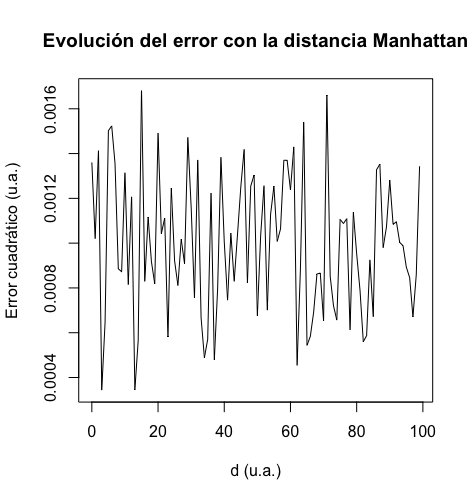
\includegraphics[width=7truecm]{Rplotmanh.png}
%     \caption{Error as a function of distance in arbitrary units.}
%     \label{fig:my_label}
% \end{figure}

\chapter{Conclusions and Future Works}

This chapter must include:
\begin{itemize}
\item A description of the conclusions of the work:
\begin{itemize}
    \item Once the results have been obtained, what conclusions are drawn?
    \item Are these results as expected? Or have they been surprising? Why?
\end{itemize}
\item A critical reflection on the achievement of the objectives initially set:
\begin{itemize}
    \item Have all objectives been achieved? If not, why?
\end{itemize}
\item A critical analysis of the monitoring of planning and methodology throughout the project:
\begin{itemize}
    \item Has the schedule been followed?
    \item Has the planned methodology been adequate?
    \item Has it been necessary to introduce changes to ensure the success of the work? Why?
\end{itemize}
\item From the impacts foreseen in \ref{s:etic}, an evaluation of whether negative impacts have been mitigated or positive impacts have been achieved.
\item If unforeseen impacts have appeared, an evaluation of how they have been managed.
\item The future lines of work that have not been explored and remain pending.
\end{itemize}

\chapter{Glossary}

\begin{description}
\item[API] Application Programming Interface. A set of protocols enabling communication between software components.
\item[ASR] Automatic Speech Recognition. The task of converting spoken audio to text.
\item[BiLSTM] Bidirectional Long Short-Term Memory. A recurrent network that processes a sequence in both directions.
\item[CIDEr] Consensus-based Image Description Evaluation. A metric that compares generated text with references using TF-IDF-weighted n-grams.
\item[CTR] Click-Through Rate. The ratio of clicks to thumbnail impressions.
\item[Diarization] The task of determining which speaker is active at each moment of a recording.
\item[F1@5s] F1 score of predicted boundaries, counting a prediction as correct if it is within 5 seconds of a reference boundary.
\item[GGUF] File format for quantised language models used by llama.cpp.
\item[GPU] Graphics Processing Unit. A processor suited to parallel computation, used here for model inference and training.
\item[JWT] JSON Web Token. A signed token used for stateless authentication.
\item[LLM] Large Language Model. A neural language model with billions of parameters trained on large text corpora.
\item[OAuth] An authorisation protocol that grants an application limited access to a user's account.
\item[ORM] Object-Relational Mapping. A technique for translating between database relations and programming language objects.
\item[$P_k$] Probabilistic segmentation error metric: the probability that two positions at a fixed distance are wrongly classified as belonging to the same or different segments.
\item[Quantisation] Representation of model weights with fewer bits (e.g.\ 8 or 4) to reduce memory and computation.
\item[RTF] Real-Time Factor. Processing speed expressed relative to the duration of the audio.
\item[SHAP] SHapley Additive exPlanations. A method that attributes a prediction to its input features.
\item[SRT] SubRip Text. A subtitle file format containing timestamped text segments.
\item[VAD] Voice Activity Detection. Detection of the parts of an audio signal that contain speech.
\item[VOD] Video-on-Demand. A media distribution model allowing users to access video content on request.
\item[VRAM] Video RAM. The memory of the GPU.
\item[WebVTT] Web Video Text Tracks. The W3C subtitle format used by HTML5 video.
\item[WER] Word Error Rate. The proportion of word substitutions, deletions and insertions in a transcript relative to a reference.
\end{description}


\bibliographystyle{IEEEtran}
\bibliography{references}

\newpage
\appendix

\section*{Appendix A: Environment Configuration}

The back end is configured through environment variables loaded with Pydantic Settings. Table~\ref{tab:env_vars} lists the main parameters of the core platform and the speech and chapter tools; the remaining tools follow the same convention.

\begin{table}[H]
\centering
\caption{Main environment variables and their default values.}
\label{tab:env_vars}
\small
\begin{tabular}{@{}llp{5.6cm}@{}}
\toprule
\textbf{Variable} & \textbf{Default} & \textbf{Description} \\
\midrule
\texttt{DATABASE\_URL}                     & ---                      & PostgreSQL connection string (asyncpg) \\
\texttt{JWT\_SECRET}                       & ---                      & Secret used to sign access tokens \\
\texttt{JWT\_EXPIRE\_MINUTES}              & \texttt{720}             & Access token lifetime \\
\texttt{STORAGE\_BASE\_PATH}               & \texttt{../uploads}      & Root of the local file storage \\
\texttt{REDIS\_URL}                        & ---                      & Redis broker of the job queue \\
\texttt{WORKER\_JOB\_TIMEOUT\_SECONDS}     & \texttt{10800}           & Maximum duration of a job \\
\texttt{WHISPER\_MODEL}                    & \texttt{large-v3-turbo}  & Whisper model \\
\texttt{WHISPER\_DEVICE}                   & \texttt{cuda}            & \texttt{cuda} or \texttt{cpu} \\
\texttt{WHISPER\_COMPUTE\_TYPE}            & \texttt{int8}            & CTranslate2 quantisation \\
\texttt{HF\_TOKEN}                         & ---                      & Hugging Face token for the gated diarization model \\
\texttt{DIARIZATION\_DEVICE}               & \texttt{cuda}            & Device for pyannote \\
\texttt{DIARIZATION\_EMBEDDING\_BATCH\_SIZE} & \texttt{8}             & Embedding batch size (GPU memory) \\
\texttt{DIARIZATION\_HEALTHCHECK}          & \texttt{true}            & Start-up health check \\
\texttt{CHAPTERS\_MODEL\_DIR}              & ---                      & Exported chapter model bundle \\
\texttt{CHAPTERS\_DEVICE}                  & \texttt{cpu}             & Device for the chapter models \\
\bottomrule
\end{tabular}
\end{table}

\end{document}
